\documentclass{article}

\usepackage[final]{style}
\usepackage[utf8]{inputenc}
\usepackage[T1]{fontenc}
\usepackage{amsmath, amssymb, amsfonts}
\usepackage{graphicx}
\usepackage{subcaption}
\usepackage{float}
\usepackage{microtype}
\usepackage{hyperref}
\hypersetup{hidelinks}

\title{STATS 305C Applied Statistics III\\Milestone 3: Latent Quality and Data-Mix Inference}
\author{Angikar Ghosal\\Stanford University \And Kaitlyn Wang\\Stanford University}
\date{}

\newcommand{\R}{\mathbb{R}}
\newcommand{\N}{\mathcal{N}}

\begin{document}
\maketitle
\vspace{-1.4em}
\small
\setlength{\parskip}{3pt}

\paragraph{Goal and data.}
The feedback on Milestone 2 asked us to make the model actionable rather than
only conclude that filters agree on some things and differ on others. We
therefore keep the original hierarchical regression as a baseline, but add a
latent-variable model whose output is a data-mix score. We use the same
120k-document modeling sample from the 2.26M-document WebOrganizer subset:
96,097 training documents, 23,903 held-out documents, 24 topics, 24 formats,
and the top 500 domains plus an ``other'' bucket. The six complete scores are
DCLM, rounded FineWeb-Edu, and PC ARC-Easy, PIQA, SciQ, and LAMBADA. Bounded
scores are clipped at $10^{-4}$, logit-transformed, and all scores/covariates
are standardized on the training split. QuRater is excluded from the likelihood
because it covers only 44 of the 100 sampled shards.

\paragraph{Generative model.}
Let $y_i\in\R^6$ be the transformed score vector and $z_i$ contain an
intercept, 17 text heuristics, topic indicators, format indicators, and domain
indicators. We fit a two-factor latent filter model:
\begin{align}
  h_i \mid z_i,\Gamma &\sim \N_2(\Gamma^\top z_i, I_2),\\
  y_i \mid h_i,\alpha,\Lambda,\psi &\sim
    \N_6(\alpha+\Lambda h_i,\operatorname{diag}(\psi)).
\end{align}
This says that filters are noisy measurements of two latent document axes whose
prior means are predicted by observable document structure. The diagonal
$\psi$ keeps filter-specific noise explicit, while $\Lambda h_i$ captures
shared cross-filter signal. We also fit a one-factor version; it mostly loaded
on DCLM/FineWeb/LAMBADA and left the PC benchmark cluster unexplained, so the
two-factor model is the scientifically useful specification.

\paragraph{Inference algorithm.}
We use EM, which is appropriate because the complete-data model is Gaussian.
For fixed parameters, the E-step computes the posterior
$p(h_i\mid y_i,z_i)=\N(m_i,V)$, where
\[
  V=(I+\Lambda^\top\operatorname{diag}(\psi)^{-1}\Lambda)^{-1},\quad
  m_i=V\{\Gamma^\top z_i+\Lambda^\top\operatorname{diag}(\psi)^{-1}(y_i-\alpha)\}.
\]
The M-step updates $\alpha,\Lambda,\psi$ by least squares using
$\mathbb{E}[h_i]$ and $\mathbb{E}[h_i h_i^\top]$, and updates $\Gamma$ by
ridge regression of $\mathbb{E}[h_i]$ on $z_i$ (equivalently a Gaussian prior
on the covariate effects). The two-factor EM run converged in 180 iterations.
The approximate observed-data log likelihood increased from $-746{,}210$ to
$-678{,}610$, with final increment 0.067, so the optimization was stable rather
than stopped manually.
For held-out covariate-only prediction, RMSE is 0.898; conditioning on the
observed filters gives reconstruction RMSE 0.625. We use the posterior expected
average reconstructed score as the latent data-mix score.

\begin{figure}[H]
  \centering
  \begin{subfigure}[t]{0.43\linewidth}
    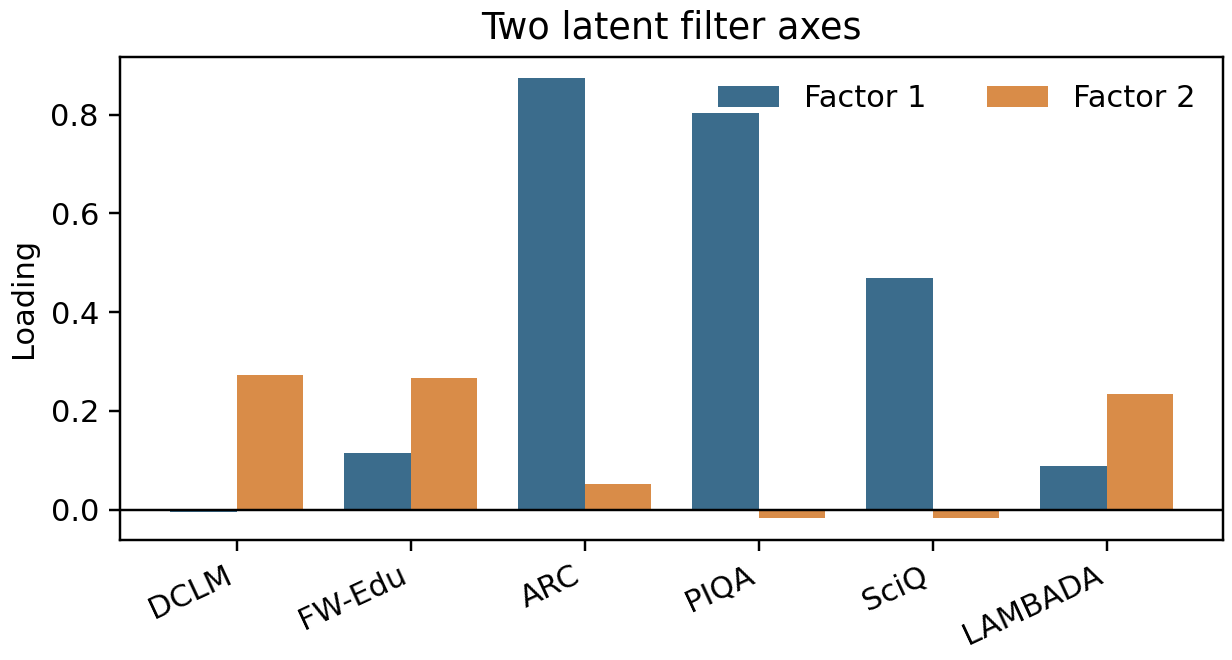
\includegraphics[width=\linewidth]{figures/week6_v2_factor_loadings.png}
    \caption{Estimated factor loadings.}
  \end{subfigure}
  \hfill
  \begin{subfigure}[t]{0.53\linewidth}
    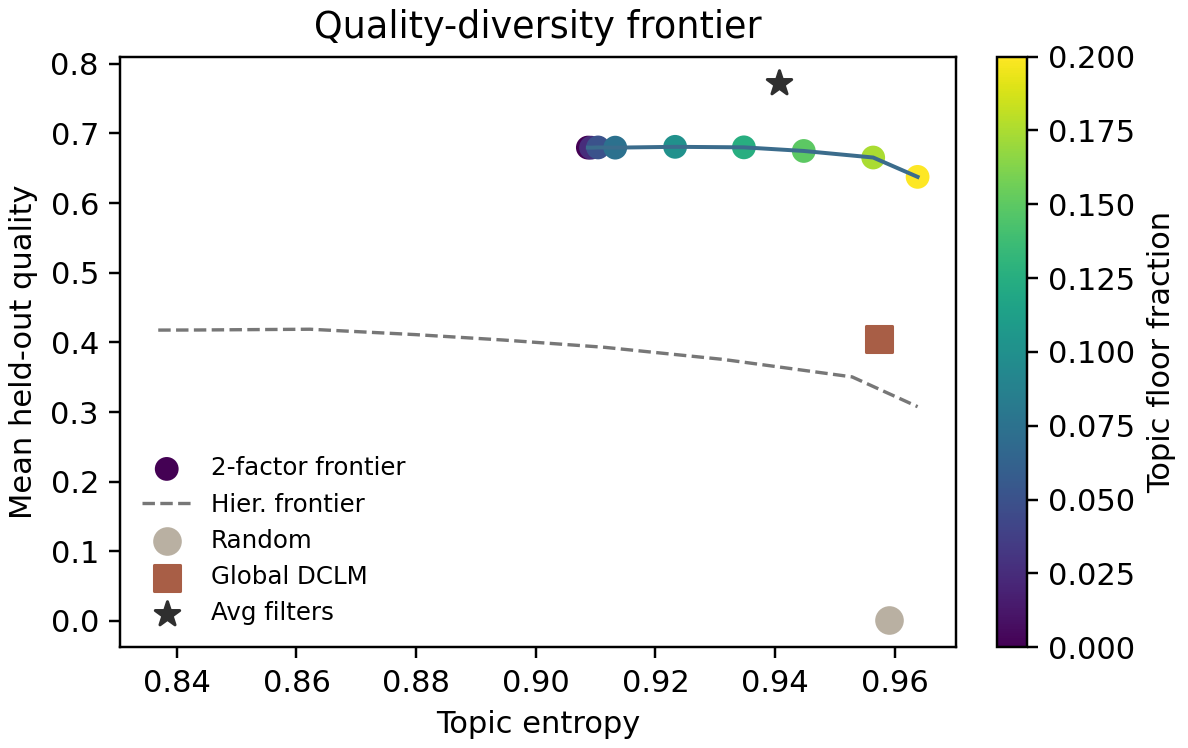
\includegraphics[width=\linewidth]{figures/week6_v2_frontier.png}
    \caption{Quality-diversity frontier.}
  \end{subfigure}
  \vspace{-0.6em}
  \caption{The EM model discovers two interpretable filter axes and produces a
  data-mix frontier that dominates the previous hierarchical regression policy.}
  \label{fig:v2-main}
\end{figure}

\paragraph{Posterior/factor analysis.}
Figure~\ref{fig:v2-main}a shows the learned loadings. Factor 1 is a benchmark
axis: ARC-Easy loads 0.87, PIQA 0.80, and SciQ 0.47. Factor 2 is a
DCLM/FineWeb/LAMBADA axis, with loadings 0.27, 0.27, and 0.23 respectively.
On the held-out set, Factor 1 correlates 0.71 with composite quality and Factor
2 correlates 0.45, so both axes matter for selection. The unique variances are
smallest for ARC-Easy (0.064) and PIQA (0.186), meaning the benchmark axis is
highly coherent, while DCLM, FineWeb-Edu, SciQ, and LAMBADA retain more
filter-specific noise.
Thus the model gives a sharper version of the Milestone 2 EDA: there is not a
single universal quality filter, but there are two coherent latent axes. This
also explains why the earlier single-response hierarchical regression improved
prediction only slightly: averaging all filters collapses these two axes too
early, while the factor model keeps both and recombines them only at the final
decision stage.

\paragraph{Baseline comparison and actionability.}
We evaluate top-20\% selection policies on held-out documents using the average
of the six standardized scores as composite quality. Random selection has mean
quality 0.001. Global DCLM reaches 0.405 with topic entropy 0.957. The previous
hierarchical topic-floor policy reaches only 0.419, and its bootstrap
difference from DCLM has a 95\% interval crossing zero. The one-factor posterior
policy improves to 0.448. The two-factor posterior policy reaches 0.680, and
the two-factor topic-floor policy reaches 0.680 with all 24 topics covered and
topic entropy 0.910. The simple average of all six filters is an upper-bound
reference at 0.772; our model does not beat this tautological score, but it
gives an interpretable probabilistic decomposition and a tunable data-mix
frontier. We also separate two use cases: if only metadata and heuristics are
available, the two-factor prior score is only 0.395 and does not improve on
DCLM; if the six filters are available, the posterior score denoises and
rebalances them. Thus the practical workflow is to score candidate documents
with the available filters, infer posterior latent axes, and choose a mixture
from the frontier rather than trusting a single global ranker.

\begin{figure}[H]
  \centering
  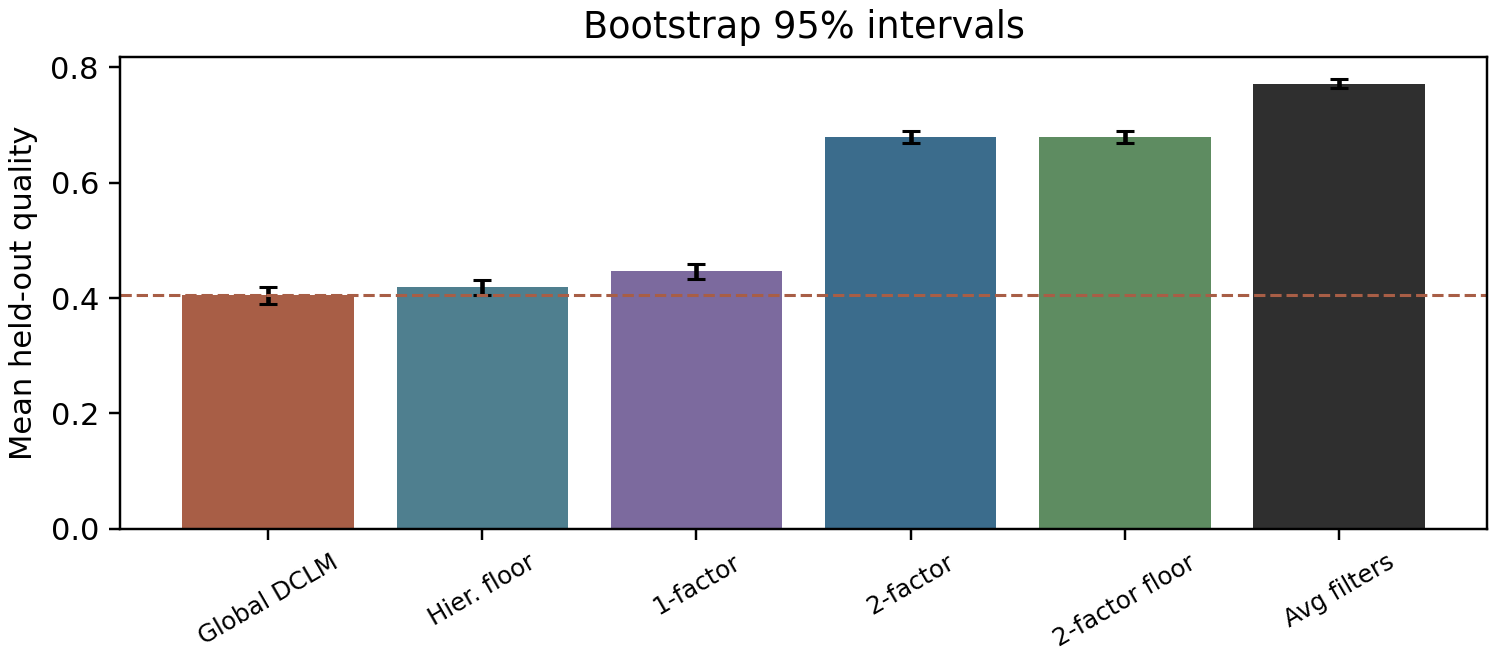
\includegraphics[width=0.72\linewidth]{figures/week6_v2_robustness.png}
  \vspace{-0.8em}
  \caption{Bootstrap intervals over held-out rows. The old hierarchical policy
  is not clearly better than DCLM, but the two-factor policies are.}
  \label{fig:v2-robust}
\end{figure}

\paragraph{Quality-diversity result.}
Figure~\ref{fig:v2-main}b varies the within-topic floor. At a 20\% floor, the
two-factor model reaches topic entropy 0.964, matching within-topic DCLM-level
diversity, while still achieving quality 0.638, far above global DCLM's 0.405.
The best frontier point is near a 10\% topic floor: quality 0.681 and entropy
0.923. This is the recommended default if the goal is quality with some topic
protection; the 20\% floor is the safer choice if the pretraining mixture must
look closer to the full corpus topic distribution.
The bootstrap improvement of the two-factor topic-floor policy over DCLM is
0.274 standardized units, with 95\% interval $(0.261,0.291)$
(Figure~\ref{fig:v2-robust}). This directly answers the feedback: the model
does something the EDA cannot. It estimates latent filter axes, then exposes a
quality-diversity frontier for choosing a pretraining data mix.

\paragraph{Limitations.}
This still evaluates against held-out filter scores, not downstream LM loss.
The next validation should train tiny language models on DCLM, average-filter,
and two-factor-frontier mixtures at matched token budgets, then compare
validation loss and benchmark accuracy. The posterior policy also uses the same
six filters that define the composite target, so it should be interpreted as a
principled smoothing and decomposition method, not proof that the composite is
the right objective. Also, FineWeb-Edu is rounded ordinal and should eventually
use an ordinal likelihood; QuRater should enter once all sampled shards are
scored.

\paragraph{Reproducibility.}
The repository contains the full pipeline in numbered experiment scripts:
factor EM fitting, policy evaluation, quality-diversity frontiers, bootstrap
intervals, and figure generation. We fixed train/test splits and random seeds,
stored generated artifacts separately from source code, and used the compiled
figures in this report directly from those local runs. The experimental branch
also contains staged commits for each modeling step, matching the milestone
requirement that repository history document progress.

\paragraph{AI assistance.}
We used Codex and Claude Code for code generation, debugging, and report
drafting. Numerical claims were checked against locally generated artifacts.

\end{document}
